\chapter{\label{chap:konzeption}Konzeption}
Die erarbeiteten Anforderungen zur Untersuchung der Konfliktmanagementstrategien offlinefähiger Systeme werden in diesem Kapitel für die Konzeption angewendet.\\
Es soll für jede zu untersuchende Technologie ein Prototyp entwickelt werden. Im Rahmen dieser Arbeit entsteht ein Prototyp der \sc{Redux Offline} verwendet und ein zweiter in dem PouchDB und CouchDB eingesetzt wird. Für letzteren könnte genauso gut HOODIE benutzt werden, da HOODIE sowohl PouchDB als auch CouchDB benutzt~\cite{hoodie-how}.
Doch da für den zu entwickelnden Prototyp lediglich diese beiden Komponenten benötigt werden, wurde sich dagegen entschieden.
Bis zu einem gewissen Status, nämlich dem der Verwendung der Technologien, sind beide Prototypen -- bis auf den Namen-- identisch.
% Beginnend mit dem Aufbau der exemplarischen Anwendung werden in den folgenden Abschnitten die  der Anwendungsaufbau, Architektur  und schließlich \todo{blabla} die graphische Oberfläche aufgeführt.
% Den Raum aller möglichen Lösungen anhand der Anforderungen auf die in irgendeinem Sinn beste / geeignetste einzuschränken:\\
% App entwickeln, in der es einen `Verbindung unterbrechen` Knopf gibt ', oder ob es aus irgendwelchen Erwägungen notwendig sein könnte, das über eine separate Instanz zu machen.
%
% Aufbau
%
\section{Anwendungsaufbau}
Die Prototypen bestehen im Frontend aus React und wurden mit \sc{Create React App} erstellt. \sc{Create React App} erstellt ein Projekt mit dem gewünschten Namen, generiert eine initiale Projektstruktur (vgl. \autoref{fig:init}) und installiert die dafür benötigten Abhängigkeiten~\cite{create-react}.
\begin{figure}[H]
  \centering
  \begin{subfigure}[t]{0.4\textwidth}
          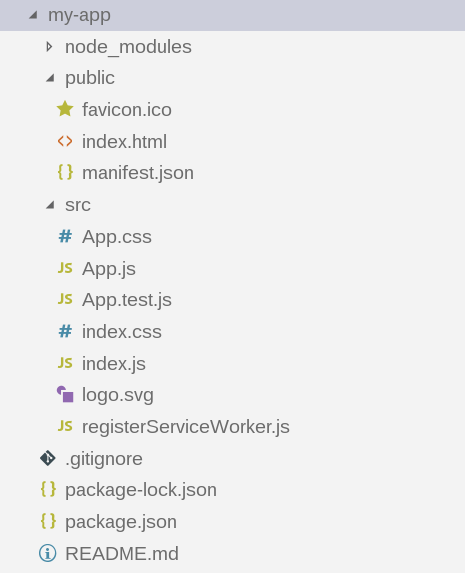
\includegraphics[width=\textwidth]{Ordnerstruktur}
          \caption{Die initiale Projektstruktur}
          \label{fig:init}
  \end{subfigure}
  ~ 
  \begin{subfigure}[t]{0.4\textwidth}
          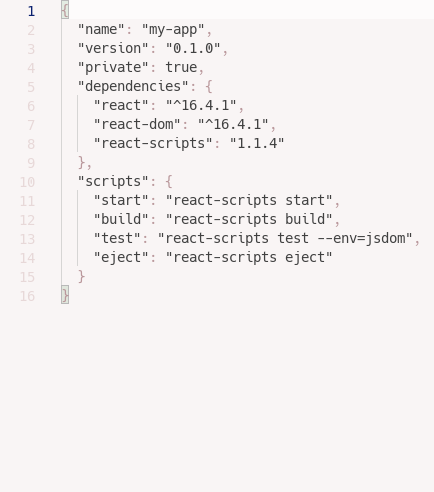
\includegraphics[width=\textwidth]{rca-package}
          \caption{Die initiale package.json Datei}
          \label{fig:init2}
  \end{subfigure}
  \grayRule
  \caption[Create React App: initiale Testapplikation]{einer mit Create React App erstellten Testapplikation}
  \label{fig:create-react-app}
\end{figure}
%
Diese sind im Verzeichnis node\_modules installiert.
Außerdem ist ein ServiceWorker
%und ein App Manifest (\tt{manifest.json}) enthalten, wodurch die \gls{PWA}-- Kriterien erfüllt sind.
enthalten der die \gls{Assets} cacht.
Als Template gibt es nun die \tt{public/index.html}-- Datei. In der \tt{index.js}--Datei werden die React--Komponenten und der ServiceWorker initialisiert. 
Alle \tt{App.*}--Dateien umfassen eine minimale Beispielanwendung.
In der generierten \tt{package.json}--Datei (vgl. \autoref{fig:init2}), befinden sich Informationen über die Anwendung und ihre Abhängigkeiten. Im Unterpunkt \tt{scripts} werden Kommandozeilen-Aufrufe definiert und können mit dem Befehl \tt{npm run} aufgerufen werden.
%
% React Komponenten
%
\sub{Aufbau der React Komponenten ?}
React ist eine open-source Bibliothek, die dazu dient, die View-Komponente des Model-View-Controller-Ansatzes abzudecken, also die Seite der Anwendung die für die Anzeige und Interaktion zuständig ist. Ein Vorteil von React sind die wiederverwendbaren Komponenten. Eine Komponente ermöglicht die Aufteilung der \gls{UI} in kleine Teile und ist eine abstrakte Basisklasse. Einmal implementiert, lässt sich eine Komponente immer wieder verwenden~\cite{react}.\\
Eine Komponente kann einen internen \tt{state} besitzen, oder die Daten nur aus den \tt{props} nehmen. \tt{Props} sind Eigenschaften die übergeben werden und nur von der Elternkomponente änderbar.
Zur Veranschaulichung wird anhand des Listings \ref{code:react-form} die reduzierte Version der Formularkomponente beider zu entwickelnden Prototypen beschrieben. In dieser Version wird nur der Name des Kontakts gezeigt und verändert.\\
Die Formularkomponente hat Kontaktobjekt im internen \tt{state} gespeichert. Auf dieses Objekt haben andere Komponenten keinen Zugriff und es ist nur via \tt{setState()} änderbar.
Initial wird das Kontaktobjekt über die \tt{props} geladen (Zeile vier). So kann das Vorausfüllen der Eingabefelder realisiert werden.\\
In Zeile sieben ist die \tt{handleChange()} Funktion, die am Eingabefeld (Zeile 22) auf die Änderungen reagiert (Zeile zehn) und der interne \tt{state} aktualisiert (Zeile 12).\\
Eine React Komponente hat immer eine \tt{render()}--Funktion (Zeile 15) die die Daten aus dem \tt{state} oder den \tt{props} liest und zurückgibt was dargestellt werden soll. Hier wird das zur Komponente gehörende \gls{HTML} erzeugt. Jede Änderung des \tt{states} führt einen erneuten Aufruf der \tt{render()}--Funktion mit sich.
% listing
\begin{center}
  \lstinputlisting[language=REACT,
  numbers=left,xleftmargin=20pt,framexleftmargin=15pt,
  caption={Limitierte Version der React Komponente \tt{ContactForm} beider Prototypen},
  label=code:react-form]{code/Form.js}
\end{center}
%
In der Elternkomponente \tt{Contacts} wird die Formularkomponente so wie es im folgenden Listing zu lesen ist, aufgerufen. Alle im Formular verfügbaren Eigenschaften werden hier übergeben.
\lstset{language=REACT,
caption={Aufruf der React \tt{ContactForm} Komponente},
label=code:form-call}
\begin{lstlisting}
  <ContactForm contact={editView.contact}
    addOrEditContact={this.addContact}
    handleCancel={this.toggleEdit} />
\end{lstlisting}
%
% Redux
%
\sub{Erweiterungen für \sc{amilia-rdx}}
Redux Offline kann nur zusammen mit Redux verwendet werden. Deswegen ist für diesen Prototypen die Implementierung von Redux vorausgesetzt.
\subsub{Redux}
Redux ist eine Bibliothek zur Zustandsverwaltung in JavaScriptanwendungen.
Mit Redux hat jede Applikation genau einen \tt{store}. Dieser hat den Applikationsstatus, der via \tt{dispatch()} aktualisiert, und via \tt{getState()} gelesen werden kann.
Als einzige Informationsquelle für den \tt{store} dienen Aktionen. Sie senden Daten von der Anwendung mittels \tt{store.dispatch()} an den \tt{store} und beschreiben dabei nicht wie etwas passiert, sondern was passiert.\\
Der dritte wichtige Bestandteil von Redux sind die \tt{Reducer}. Sie spezifizieren wie der Status sich als Reaktion auf die Aktionen ändert~\cite{redux}.
% % Der Datenfluss in der Reduxarchitektur ist unidirektional.
% Zur Veranschaulichung des Datenflusses in Redux wird anhand des Listings \ref{code:redux-dataflow} das Wechseln der Ansichten Liste und Formular beschrieben.
% Alles beginnt mit dem Aufruf von \tt{store.dispatch(action)} von jeder beliebigen Stelle in der Anwendung. Die Aktion die beschreibt was passiert heißt \tt{toggleEdit} und sieht im Beispiel des Ansichtswechsels aus wie in Zeile drei bis fünf.\\
% Der \tt{Store} ruft nun den \tt{Reducer} auf
% % listing
% \begin{center}
% \lstinputlisting[language=REACT,
% numbers=left,xleftmargin=20pt,framexleftmargin=15pt,
% caption={Datenfluss in Redux},
% label=code:react-form]{code/Redux.js}
% \end{center}
\subsub{Redux Offline}
Redux Offline ist eine erweiternde Bibliothek für Redux dessen Funktionsweise in Abschnitt \ref{sub:reduxoffline} detailliert beschrieben wird.\\
Nach der Installation muss der Redux \tt{store} zusammen mit dem \tt{offline "-store "-enhancer} erzeugt werden. Listing \ref{code:store} visualisiert diesen Vorgang. Ein Redux \tt{store} wird mit dem \tt{storeCreator} in Zeile fünf erzeugt. Ein \tt{store "-enhancer} ist eine Funktion die den \tt{storeCreator} neu zusammenfügt und einen neuen, erweiterten \tt{storeCreator} zurückgibt.
Redux Offline kommt mit einer vorgegebenen Konfiguration (siehe Zeile 3). Diese wird dem \tt{offline store enhancer} in Zeile acht übergeben.
\begin{center}
  \lstinputlisting[language=REACT,
  firstline=53,lastline=62,
  numbers=left,xleftmargin=20pt,framexleftmargin=15pt,
  caption={Erstellen eines Stores mit Redux Offline},
  label=code:store]{code/Redux.js}
\end{center}
Der gesamte Kontext der zum Synchronisieren einer Aktion erforderlich ist in einem zusätzlichen Metaattribut gespeichert. Damit die Anwendung weiß wie die Aktionen verarbeitet werden sollen wird sie mit dem Metafeld dekoriert. Die Aktion zum Lesen der Kontakte könnte dann wie im folgenden Listing aussehen.
%
\begin{center}
  \lstinputlisting[language=REACT,
  firstline=9,lastline=20,
  numbers=left,xleftmargin=20pt,framexleftmargin=15pt,
  caption={Aktion \tt{fetchContacts} mit Metaattribut},
  label=code:react-meta]{code/Redux.js}
\end{center}
%
Das erste \tt{meta.offline} Feld beschreibt die Netzwerkaktion die ausgeführt werden soll, also den Aufruf an die angegebene URL in Zeile sechs. Bei \tt{commit} in Zeile sieben wird festgelegt welche Aktion bei erfolgreichem Netzwerkaufruf augeführt werden soll. Für den Fall dass von dem angefragtem \gls{API} der Statuscode 500 zurückkommt oder der Server nicht läuft, wird die im \tt{rollback} definierte Aktion gefeuert.\\
Die Aktionen beschreiben nur was passiert. Wie der Status sich ändert, wird im \tt{Reducer} beschrieben. Das Listing \ref{code:reducer} illustriert wie das im entsprechendem Prototypen umgesetzt werden könnte.
%
\begin{center}
  \lstinputlisting[language=REACT,
  firstline=36,lastline=50,
  numbers=left,xleftmargin=20pt,framexleftmargin=15pt,
  caption={Reducer mit allen Aktionen die im Meta Feld beschrieben werden},
  label=code:reducer]{code/Redux.js}
\end{center}
%
In diesem Beispiel wird der Appstatus nur bei erfolgreichem Netzwerkaufruf aktualisiert. Das ist in den Zeilen sieben bis zehn nachzulesen. Und auch nur dann, wenn sich die Antwort vom Server von diesem unterscheidet.
%
%
% Architektur
%
\section{Architektur}
Die zu erstellenden Prototypen erhalten die Namen \it{amilia-qouch} und \it{amilia-rdx}, wobei Amilia der Name ist, der sich in den Beispielkontakten in den Szenarien wiederfindet. Die Abkürzung \it{rdx} steht für Redux und zeigt, dass dieser Prototyp \sc{Redux Offline} verwendet. Die Endung \tt{qouch} soll die Symbiose von CouchDB und PouchDB darstellen. Der Buchstabe Q klingt wie das hart ausgesprochene C in Couch und wenn man das kleine Q horizontal spiegelt, sieht man das P für Pouch.\\\\
Beide Prototypen setzen sich aus den nachfolgend beschriebenen Komponenten zusammen, welche in Abbildung \ref{fig:uml} veranschaulicht werden.\\\\
Die Komponente \tt{Contacts} fungiert als Container und ist das Herzstück der Anwendung. Er definiert die graphische Oberfläche und stellt alle notwendigen Funktionen bereit. Sie hat einen internen \tt{state} in dem sowohl die Kontaktliste, als auch die Daten für das Formular gespeichert sind. Im Diagramm ist der \tt{state} an der blauen Schrift zu erkennen. Das Objekt \tt{editView} zeigt, welche Ansicht -- Liste oder Formular -- gerade aktuell ist und speichert den im Formular zu ladenden Kontakt. Wie das Kontaktobjekt aufgebaut ist zeigt der blaue Kasten im Diagramm. Wird eine Aktion zum Ändern der Ansicht aufgerufen, beispielsweise durch das Betätigen eines Knopfes, wird über die Funktion \tt{toggleEdit()} der interne \tt{state} aktualisiert und ein erneutes Rendern der Komponente eingeleitet. Dann wird entsprechend die Liste oder das Formular gerendert.\\
Die \tt{Header}--Komponente zeigt den Netzwerkstatus der Anwendung an und hat einen Knopf, der zum \tt{ContactForm} führt.\\
Die \tt{ContactList} wird initial gerendert. Es werden alle Kontakte als Liste dargestellt. Hier kann das Bearbeiten (\tt{handle"-On"-Edit"-Click()}) oder das Löschen (\tt{handle"-On"-De"-lete"-Click()}) des Kontakts eingeleitet werden.
\begin{figure}[H]
  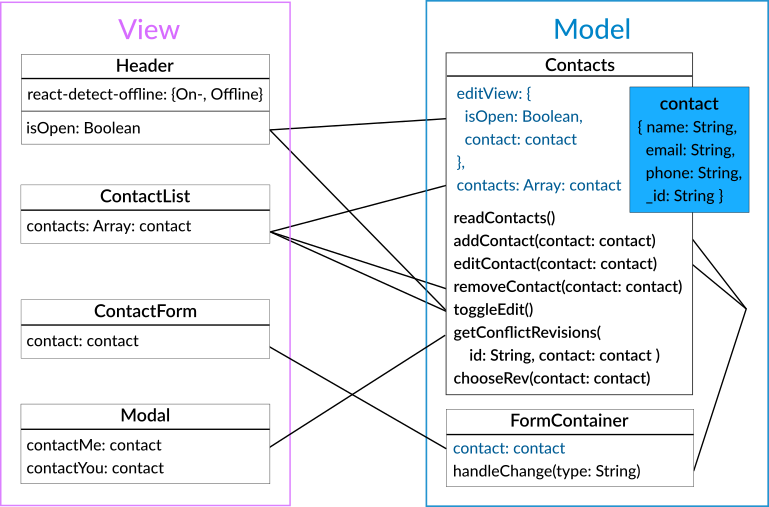
\includegraphics[width=\textwidth]{uml}
  \grayRule
  \caption{Komponentenarchitektur}
  \label{fig:uml}
\end{figure}
Die Komponente \tt{ContactForm} zeigt, sofern vorhanden, alle im Kontakt gespeicherten Daten an. Diese können hier bearbeitet werden. Gibt es keine Kontaktdaten die geladen werden kann, kann hier ein neuer Kontakt angelegt werden. Zusätzlich zu den Eingabefeldern für jedes Kontaktattribut hat sie zwei Knöpfe mit denen die Aktion bestätigt (\tt{handleSubmit()}) oder abgebrochen (\tt{handleCancel()}) werden kann. Sie ist neben \tt{Contacs} die einzige Komponente mit einem internen \tt{state}. Dieser wird für die Ereignishandler benötigt, die auf die Veränderung der einzelnen Eingabefelder zu ``lauschen``. Der zu bearbeitende Kontakt wird hier zwischengespeichert und dann als Ganzes an \tt{Contacts} gegeben.\\
\todo{Konflikt--Dialog}\\\\
%
% 
%
\todo{Backend: Implementierung bei qouch nicht notwendig. Nur Installation von Couch.\\ 
Für Redux Offline: Server der alle \gls{CRUD} Operationen unterstützt und JSON Datei zur Persisierung ( DB Ersatz?)  um Ergebnisse nicht zu verfälschen UND Redux- store, actions, Reducer}
% Client - Server - Modell
\begin{figure}[H]
  \centering
  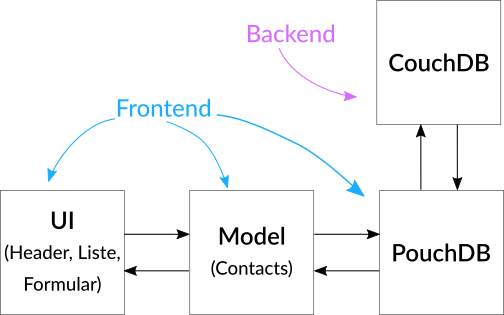
\includegraphics[width=0.6\textwidth]{qouch-model}
  \grayRule
  \caption{Client-Server-Modell}
  \label{fig:qouch-model}
\end{figure}
%
% Speicherung & Sync
%
\sub{\label{chap:persist}Das Speichern der Daten}
Das Seichern von Kontakten wird in den Prototypen unterschiedlich implementiert.
%
% --------------------------------------------------------------------------------- Qouch
%
\subsub{Daten mit PochDB und CouchDB speichern}
Für den Protoyp \it{amilia-qouch} muss zunächst CouchDB installiert werden.
% sudo apt-get install couchdb
Sobald dieser Schritt erledigt ist läuft CouchDB auf \tt{localhost:5984} und ist einsatzbereit.
Das asynchrone \gls{API} von PouchDB stellt alle notwendigen Funktionen bereit die sowohl Callbacks, Promises als auch asynchrone Funktionen unterstützen. 
Das Listing \ref{code:pouch} führt alle benötigeten Funktionen auf und zeigt die notwendigen Schritte zur Synchronisation der lokalen PouchDB und CouchDB.\\
Die lokale Datenbank wird in Zeile zwei erstellt. Wenn es die Datenbank mit dem Namen `contacts` bereits gibt, wird sie gestartet.\\
Um eine CouchDB Instanz zu erzeugen ist der Aufruf in Zeile drei mit der URL zur Couch"-DB--Datenbank notwendig. Auch hier erstellt PouchDB die Datenbank, sofern sie noch nicht existiert. PouchDB funktioniert nun als Client zu einer online CouchDB Instanz.
Zur kontinuierlichen Synchronisation beider Instanzen, der lokalen PouchDB und der Couch"-DB, ist lediglich der Aufruf in Zeile fünf erforderlich. Im optionalen Parameter können zum Beispiel FIlter oder Einstellungen zum wiederholten Synchronisationsversuch im Falle eines Fehlschlags gesetzt werden ~\cite{pouch_options}.\\
% GET
Der Aufruf \tt{localDB.allDocs()} in Zeile acht fragt alle in der lokalen Datenbank gespeicherten Kontakte an.
Ohne den Parameter \tt{include\_docs: true} werden nur die ID, \tt{\_id} und die Revisionsnummer, \tt{\_rev} eines jeden gespeicherten Kontakts zurückgegeben.
Ist die Option \tt{conflicts} auf \tt{true} gesetzt, werden Konfliktinformationen zu jedem Kontakt gespeichert. Alle konfliktbehafteten Kontakte haben nun ein \tt{\_conflicts} Attribut. Dort bedindet sich eine Liste mit allen konkurrierenden Revisionen.\\\\
%
Für die nachfolgenden Aufrufe gibt es mehrere Varianten. Eine Anleitung zu dem Umgang mit Konflikten in der PouchDB Dokumentation empfiehlt für das Erstellen, Aktualisieren und Löschen eines Dokuments das Modul PouchDB Upsert zu verwenden. Das wird in Zeile eins zu, PouchDB Objekt hinzugefügt. Jedes Mal wenn eine der \gls{CRUD} Operationen auf einem Dokument ausgeführt wird und das \gls{API} eine Revision verlangt, kann ein Konfliktfehler geworfen werden. Zum praktischen Umgang empflieht PouchDB die Aktion zu wiederholen, bis sie erfolgreich war.
Dazu kann PouchDB Upsert verwendet werden. Es fügt ein neues Dokument hinzu wenn noch keins existiert und aktualisiert es, wenn es vorhanden ist ~\cite{pouch_conflicts}. Konflikte treten so trotzdem auf und CouchDB wählt eine gewinnende Version aus. Alle Konflikte werden immenrnoch gespeichert und die beteiligten Dokumente können wie oben beschrieben aus der CouchDB geladen werden.\\
%
\begin{center}
  \lstinputlisting[language=REACT,
  numbers=left,xleftmargin=20pt,framexleftmargin=15pt,
  caption={Persistierung der Daten mit PouchDB und CouchDB}, 
  label=code:pouch]{code/Pouch.js}
\end{center}
%
% CREATE
Die Zeilen 13 bis 16 zeigen wie ein Kontakt erzeugt werden kann. Bevor das geschieht wird eine ID erstellt die aus dem aktuellen Zeitstempel besteht. Diese wird dann per PouchDB Upsert in dem neuen Dokument gespeichert.\\
% Bei dessen Verwendung wird \tt{\_id} von PouchDB automatisch generiert. Diese Variante wird jedoch nicht empfohlen, weil dann die IDs zufällig sind, die Objekte nicht danach sortiert werden können~\cite{pouch-create}.\\
% UPDATE
Das Aktualisieren eines Kontakts sieht sehr ähnlich aus, da die \tt{upsert} Funktion für beide Operaktionen verwendet wird.
% Zuerst wird der entsprechende Kontakt wie in Zeile zwölf aus der Datenbank angefragt um dann in der Datenbank aktualisiert zu werden.
Mit jedem Update bekommt ein Kontakt von PouchDB eine neue Revision.\\
% DELETE
Man kann einen Kontakt mit PouchDB Upsert wie in Zeile 35 löschen.
Der Kontakt nicht wirklich gelöscht sondern wird durch ein \tt{\_deleted} Attribut als solches markiert.
%Dann ist das Kontaktdokument mit all seinen Feldern gelöscht. Die lokale Datenbank soll sich mit CouchDB synchronisieren. Ist die Revision eines gelöschten Kontakts nicht mehr vorhanden, kann diese nicht repliziert werden. Deswegen wird der Kontakt wie in Zeile 19 als gelöscht markiert und aktualisiert.
%
% Redux Offline
%
\subsub{Daten mit Redux Offline speichern}
Die Idee hinter Redux Offline ist, dass der Redux Store die lokale Datenbank ersetzt. Sobald der Appstatus sich ändert, also irgendwo im Code \tt{setState()} ausgeführt wird, wird er automatisch lokal gespeichert. Dazu wird intern \tt{redux-persist} benutzt, dessen Funktionsweise in Abschnitt \ref{sub:reduxpersist} erläutert wird. Der Redux Store wird bei jeder Änderung persistiert und beim Start der Anwendung neu geladen.
% Es bedarf keiner zusätzlichen Implementierung für die lokale Speicherung der Kontaktdaten.\\
Wie die Daten mit Redux Offline gespeichert synchronisiert werden ist am folgenden Listing erklärt.
\begin{center}  \lstinputlisting[language=REACT,
  numbers=left,xleftmargin=20pt,framexleftmargin=15pt,
  caption={Speicherung der Daten mit Redux Offline}, 
  label=code:syncrdx]{code/Redux-sync.js}
\end{center}
%
Mit dem Aufruf der Aktion ADD\_CONTACT wird der Vorgang gestartet einen Kontakt hinzuzufügen. Die anzufragende URL ist im \tt{meta.offline.effect} Feld in Zeile neun festgelegt. Die Anfrage geht an den Server, welcher die Daten in der \gls{JSON} Datei persisitiert.
Der Reducer hat Zugriff auf das Aktionsobjekt. Dort ist der gerade hinzugefügte Kontakt gespeichert. Mit diesem wird in Zeile 23 der Appstate aktualisiert und so lokal gespeichert.\\
Ist die Netzwerkanfrage erfolgreich, wird die Aktion \tt{commit} in Zeile zwölf gefeuert. Die wird im Reducer in Zeile 25 behandelt. Der \tt{state} wird mit der Antwort vom Server aktualisiert und die Synchronisation ist vollzogen.\\\\
Wie die Serverimplementierung für den gerade beschriebenen Fall aussehen könnte, beschreibt das Listing \ref{code:server}.
%
\begin{center}  \lstinputlisting[language=REACT,
  numbers=left,xleftmargin=20pt,framexleftmargin=15pt,
  caption={Mögliche Serverimplementierung für das Hinzufügen eines Kontakts}, 
  label=code:server]{code/Server.js}
\end{center}
%
In Zeile zwei werden die Kontakte aus einer \gls{JSON} Datei geladen. Diese sind als Objekt in einem Array gespeichert. Bekommt der Server eine post--Anfrage, wird ein Kontaktobjekt mitgesendet. Dieser wird in Zeile fünf in einer Variable zwischengespeichert. 
Wird der Kontakt korrekt gesendet wird er in Zeile zehn dem Array hinzugefügt. Andererseits sendet der Server den \gls{HTTP}--Statuscode 400 an den Client. % bad request
Außerdem wird mithilfe des in Node integriertem Dateisystem\footnote{siehe hierzu: \url{https://nodejs.org/api/fs.html}} Moduls die \gls{JSON} Datei neu geschrieben. Nun ist der neue Kontakt persistiert. Kommt es beim Schreiben der Datei zu keinem Fehler, sendet der Server den frisch gespeicherten Kontakt zurück an den Client.
% -----------------------------------------------------------------------------
%
% Online / Offline
%
\sub{Verbindungsstatus feststellen und ändern}
Für die Überprüfung der Verbindung zum Server wird das Modus \sc{React Detect Offline} verwendet. Es beobachtet den Online-- und Offlinestatus und bietet zwei Komponenten entsprechend des Status den Inhalt rendern. Der folgende Codeausschnitt zeigt eine Verwendung dieser beiden Komponenten. Ist die Anwendung online, wird `you are online` gerendert. Im anderen Fall ~`you are offline`.
%
\begin{center}
\lstinputlisting[language=REACT,caption={Beispiel einer React Detect Offline Implementierung}, label=code:react-detect]{code/Header.js}
\end{center}
%
Das Modul fragt alle fünf Sekunden die URL \url{https://ipv4.icanhazip.com} ab und rendert je nach Verbindungsstatus die entsprechende Komponente. Verschiedene Parameter wie die URL oder das Poll--Interval können konfiguriert werden~\cite{react-detect}.\\\\
%
Der Verbindungsstatus kann im Browser geändert werden. Die Prototypen, die im Rahmen dieser Arbeit entwickelt werden, sollen in den Browsern Firefox und Chromium laufen.\\
In Firefox lässt sich der Netzwerkstatus über das Einstellungsmenü ändern. Dort kann man entweder unter dem Punkt `Sonstiges` oder dem Punkt `Web-Entwickler` `Offline arbeiten` auswählen und ist vom Internet getrennt. Dieser Status lässt sich über den selben Weg rückgängig machen.\\
In Chrome öffnet man dazu die Entwicklertools, geht auf `Netzwerk` und klickt auf die Checkbox `Offline` am oberen Rand. Dieselbe Checkbox ist auch im `Application`--Tab unter `Service Workers` zu finden.
%
% UI
%
\section{Die graphische Oberfläche}
Aus den minimalen Anforderungen an die graphische Oberfläche ergibt sich das Design.
Anhand der folgenden Abbildungen werden die gefertigten Entwürfe der BenutzerInnenoberfläche dargestellt.\\\\
Diese Listenansicht in Abbildung \ref{fig:list} besteht aus dem Header / Kopf und den Listeneinträgen.
Sie zeigt die Kontakteinträge in beiden Netzwerkstatus: online (Abbildung \ref{fig:list-online}) und offline (\ref{fig:list-offline}).\\\\
%
%
Im Header ist abzulesen, ob die Anwendung gerade eine Verbindung zum Server hat oder nicht.
Für eine bessere Prägnanz wurden hierzu unterstützend die Farben Rot für keine Verbindung und Grün für eine bestehende Netzwerkverbindung gewählt.
Rechts im Header gibt es einen Knopf, mit dem man in die Ansicht gelangt, in der ein Kontakt hinzugefügt werden kann.\\
%
In der Liste sieht man die Namen der Person und jeweils einen Knopf zum Bearbeiten oder Löschen.
Mit der Betätigung des ''Delete''--Knopfes wird der entsprechende Eintrag in der Liste gelöscht
\begin{figure}[H]
  \centering
  \begin{subfigure}[t]{0.49\textwidth}
          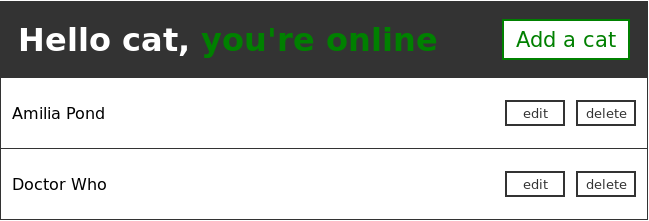
\includegraphics[width=\textwidth]{list-online}
          \caption{Kontaktliste im Onlinestatus}
          \label{fig:list-online}
  \end{subfigure}
  ~ 
  \begin{subfigure}[t]{0.49\textwidth}
          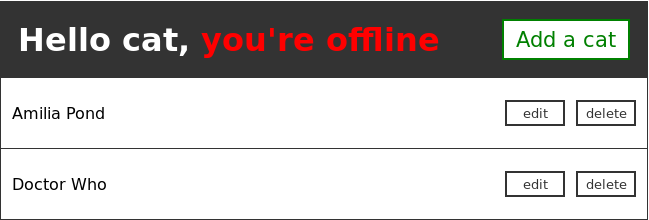
\includegraphics[width=\textwidth]{list-offline}
          \caption{Kontaktliste im Offlinestatus}
          \label{fig:list-offline}
  \end{subfigure}
  \grayRule
  \caption{Die Kontaktliste in beiden Netzwerkstatus}
  \label{fig:list}
\end{figure}
Klickt man auf den Knopf zum Bearbeiten oder auf den zum Hinzufügen eines Kontakts, gelangt man in die Bearbeitungsansicht (vgl. Abbildung \ref{fig:edit}). Der Header ist bis auf den Knopf zum Hinzufügen eines Kontakts identisch zu dem der Liste. Auch hier ist abzulesen, ob die Anwendung on-- oder offline ist. Da man sich bereits in der Ansicht zum Anlegen oder Editieren eines Kontaks befindet, ist der Knopf im Header überflüssig.\\
Ein Kontakt hat einen Namen, eine E-Mailadresse und eine Telefonnummer. In dieser Ansicht gibt es für jedes Attribut ein Eingabefeld. Die Felder sind beim Bearbeiten des Kontakts vorausgefüllt. Mittels Betätigung des ''Speichern'' Knopfs werden die Änderungen übernommen, klickt man auf ''Cancel'', werden sie verworfen. In beiden Fällen gelangt man wieder zur Listenansicht.
\begin{figure}[H]
  \centering
  \begin{subfigure}[t]{0.49\textwidth}
          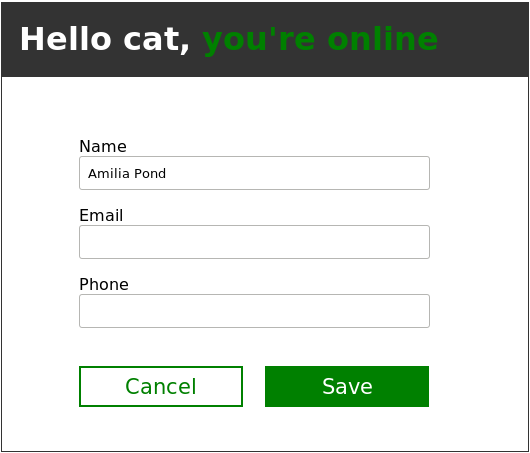
\includegraphics[width=\textwidth]{edit}
          \caption{Editieransicht im Onlinestatus}
          \label{fig:edit-online}
  \end{subfigure}
  ~ 
  \begin{subfigure}[t]{0.49\textwidth}
          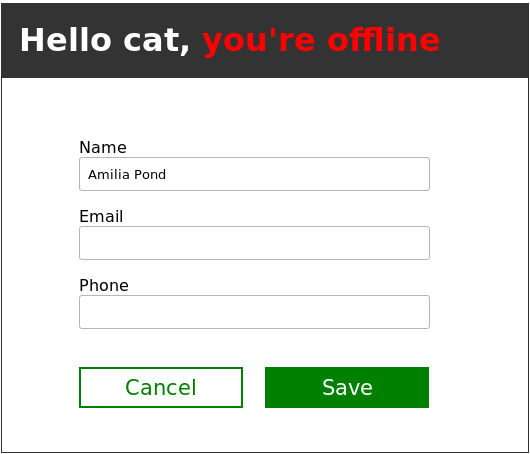
\includegraphics[width=\textwidth]{edit-offline}
          \caption{Editieransicht im Offlinestatus}
          \label{fig:edit-offline}
  \end{subfigure}
  \grayRule
  \caption{Die Editieransicht in beiden Netzwerkstatus}
  \label{fig:edit}
\end{figure}
Sobald ein Konflikt entstanden ist, soll sich ein Dialog öffnen, der die nutzenden Personen darüber informiert, welcher Kontakteintrag konfliktbehaftet ist und mit welcher Version er konkurriert.
Anhand des Dialoginhalts kann unterschieden werden, welche Version die lokal gespeicherte ist und welche vom Server kommt.
Der Dialog beinhaltet außerdem zwei unterschiedlich farbige Knöpfe, die jeweils den Kontakteintrag in einer anderen Version anzeigen.
Durch Klick auf einen Knopf wird die bevorzugte Version des Kontakts gespeichert und die andere verworfen.
So kann ein Mensch entscheiden, welche Version behalten werden soll und es wird sichergestellt, dass keine Daten verloren gehen.\\
Für die Implementierung des Konfliktdialogs ist es notwendig, dass die zu untersuchenden Technologien die Möglichkeit bieten, Konflikte zu speichern oder wenigstens als solche zu identifizieren, sodass sie manuell gespeichert werden können.
%
% Tests
%
\section{Tests}
\todo{Auch testen ob Offlinefunktionalität gewährleistet ist? -- Scope: Zeitlichen Rahmen sprengen usw.}\\
Um das Konfliktmanagement der zu testenden Technologien untersuchen zu können, müssen zunächst Konflikte erstellt werden. Dazu muss in erster Linie die Anwendunng auf mindestens zwei Geräten laufen und der Netzwerkstatus muss änderbar sein. Es ist außerdem hilfreich, wenn die Anwendung zeigt, in welchem Status sie sich befindet. Sie sollte wissen, ob sie on-- oder offline ist.\\
\todo{Kontakte editieren (auf 2 Geräten gleichzeitig) on-on, off-off, on-off? Dasselbe für Anlegen und löschen?}\\
Zur Auswertung der Daten sollten alle Ausgangspositionen, Vorgänge und Ergebnisse dokumentiert werden. Für einen Testfall kann hierfür zuerst der Kontakt aufgeschrieben werden. Dann die Operation, z.B. `bearbeiten des Kontakts Amilia` zusammen mit dem Verbindungsstatus (von Client und Server). Ebenso muss der Kontakt aufgeschrieben werden, wie er nach der Synchronisation aussieht. \todo{Lösung anbieten: .log--Datei?}
\highlight{Es stellt sich die Frage wie oft ein Testfall durchlaufen werden muss um eine sinnvolle Aussage treffen zu können}.